% !TeX root = ../UrrutiaAnguiano_CandidaturaDefensa.tex
% !TeX spellcheck = es_MX 

\section{Publicaciones y manuscritos}


{\setbeamertemplate{frametitle}[centertitle]{}
\begin{frame}{\underline{Publicaciones y manuscritos}}{}
	\begin{center}
		\begin{tikzpicture}[node distance=2.5mm and 10mm,font=\normalfont]
			%        \setlength{\leftmargini}{10pt}
			
			% caract
			\node[flowbox] (publicado) {%
				\fbtitle{
					\begin{minipage}{.425\textwidth}
						Phase Singularity in Random Gold Metasurface for Refractive Index Sensing: %
						Experimental Demonstration and Theoretical Analysis
					\end{minipage}
					}
				\nodepart{two}
				\begin{minipage}{.4\textwidth}
					\begin{itemize}
						\item	J. P. Cuanalo-Fernández, N. Korneev, I. Cosme, M. B. De La Mora, \emphr{J. A. Urrutia-Anguiano}, A. Reyes-Coronado, R. Ramos-García y  S. Mansurova\\[.5em]
						\item \textit{J. Phys. Chem. C} \textbf{128}(27): 11372–11381, 2024
						\item DOI: {10.1021/acs.jpcc.4c02274}\\[.25em]
					\end{itemize}
					\begin{center}
						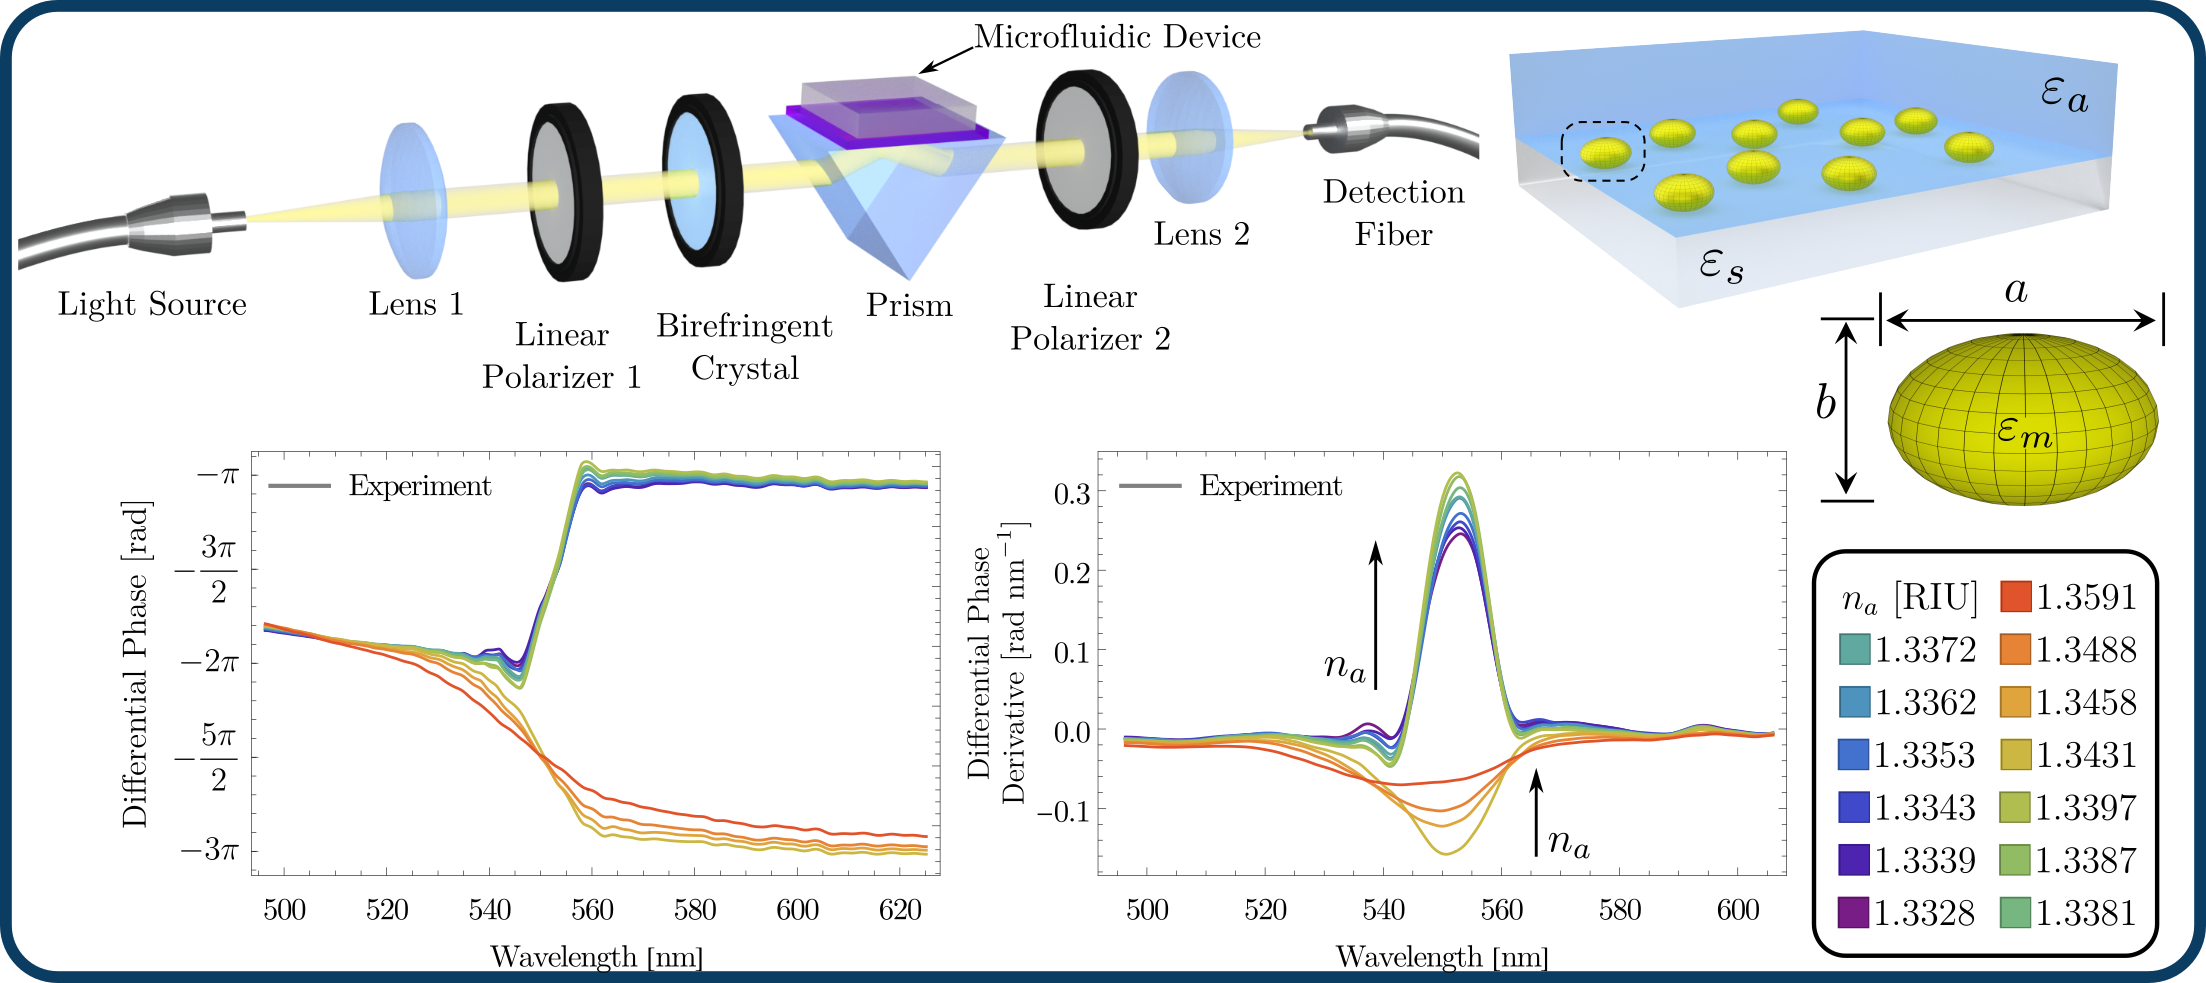
\includegraphics[scale=.45]{img/g1647.png}
					\end{center}
					\vskip.5em
				\end{minipage}
			};	
			
			\node[concept, right =of publicado, yshift=40mm] (substrate) 
				{\begin{minipage}{.425\textwidth}
				Theoretical and numerical approach to substrate effects in random plasmonic metasurfaces
				\end{minipage}};
			\node[below = of substrate] 
				{\begin{minipage}{.4\textwidth}
						\begin{itemize}
							\item \emphr{Jonathan A. Urrutia-Anguiano}, Isabel Y. Rojas-Martinez, Juan P. Cuanalo-Fernández, Alejandro Reyes-Coronado, Rubén Ramos-García y  %
							Svetlana Mansurova
							\item Revisión interna entre colaboradores
						\end{itemize}
				\end{minipage}};
			
			\node[concept, right =of publicado, yshift=-10mm] (blue) 
				{\begin{minipage}{.425\textwidth}
						Spectral shift in the strong couple regime: Red- and blueshift in plasmonic disordered metasurfaces
				\end{minipage}};
			\node[below = of blue] 
				{\begin{minipage}{.4\textwidth}
						\begin{itemize}
							\item Juan P. Cuanalo-Fernández, \emphr{Jonathan A. Urrutia-Anguiano}, Irving Gazga-Gurrión,  Nikolai Korneev, Alejandro Reyes-Coronado, Rubén Ramos-García y  %
							Svetlana Mansurova
							\item En proceso de escritura
						\end{itemize}
				\end{minipage}};
		
		\end{tikzpicture}
	\end{center}
\end{frame}
}